\documentclass[12pt]{article}
\setcounter{tocdepth}{4}
\setcounter{secnumdepth}{4}
\usepackage{amsmath,amsfonts}
\newcommand{\documento}{Piano Di Qualifica}
\usepackage{titling}
\usepackage{caption}
\usepackage{multirow}
\usepackage[T1]{fontenc}
\usepackage[utf8]{inputenc}
\usepackage[italian]{babel}
\usepackage{tabularx}
\usepackage [colorlinks=true,urlcolor=blue, linkcolor=black]{hyperref}
\newcommand{\subtitle}[1]{%
  \posttitle{%
    \par\end{center}
    \begin{center}\LARGE#1\end{center}
    \vskip0.5em}%
}

\setlength{\oddsidemargin}{0in}
\setlength{\evensidemargin}{0in}
\setlength{\topmargin}{0in}
\setlength{\headsep}{-.25in}
\setlength{\textwidth}{6.5in}
\setlength{\textheight}{8.5in}

\font\myfont=cmr12 at 40pt

\newcommand{\red}{\pie}
\newcommand{\verp}{\daL}
\newcommand{\res}{\pie}
\newcommand{\version}{Versione 2.0.0}
\newcommand{\use}{Esterno}
\newcommand{\myparagraph}[1]{\paragraph{#1}\mbox{}\\ \\}
\usepackage{eurosym}
\title{\fontsize{40}{40}\selectfont Piano di Qualifica}
\author{Dream Corp.}


\setcounter{tocdepth}{4}
\setcounter{secnumdepth}{4}
\usepackage{float}
\usepackage{wrapfig}
\usepackage{appendix}
\usepackage{amsmath, tabu}
\graphicspath{{immagini/}}
\date{07/03/2019}

\begin{document}

	\maketitle
	\begin{center}
	
\includegraphics[width = 80mm]{../../logo.png}\newline
	\huge \version 
	\\G\&B
	
	\begin{table}[h!]
		\centering
		\begin{tabular}{r|l}
			\multicolumn{2}{c}{Informazioni sul documento}\\
			\hline
			Versione & \version \\
			Redazione & \red \\
			Verifica & \verp\\
			& \vers\\
			Responsabile & \res\\
			Uso & \use\\
			Destinatari & Dream Corp. \\
			& Zucchetti SpA\\
			& Prof. Tullio Vardanega\\
			& Prof. Riccardo Cardin\\
		\end{tabular}
	\end{table}
	
	\end{center}
	\newpage
	\medskip
\begin{table}[h!]
	\centering
	\renewcommand{\arraystretch}{2} 
	\rowcolors{2}{gray!25}{white}
	\begin{tabular}{|r|r|p{6cm}|l|l|}
		\rowcolor{orange!50}		
		\hline
		\textbf{Versione} & \textbf{Data} & \textbf{Descrizione} & \textbf{Autore} & \textbf{Ruolo}\\
		\hline
		0.6.0 & 9/01/2019 & Consuntivo di periodo e preventivo a finire & \pie & Responsabile \\
		\hline
		0.5.3 & 17/12/2018 & Preventivo validazione e totali & \pie & Responsabile \\
		\hline
		0.5.2 & 15/12/2018 & Preventivo progettazione di dettaglio & \pie & Responsabile \\
		\hline
		0.5.1 & 14/12/2018 & Preventivo progettazione architetturale & \pie & Responsabile \\
		\hline
		0.5.0 & 13/12/2018 & Preventivo avvio e analisi & \pie & Responsabile \\
		\hline
		0.4.0 & 13/12/2018 & Analisi dei Rischi & \daG & Analista \\
		\hline
		0.3.1 & 12/12/2018 & Inserimento diagrammi di Gantt & \pie & Responsabile \\
		\hline
		0.3.0 & 11/12/2018 & Scrittura pianificazione & \pie & Responsabile \\
		\hline
		0.2.0 & 05/12/2018 & Scrittura modello di sviluppo  & \daG & Responsabile \\
		\hline
		0.1.0 & 30/11/2018 & Scrittura introduzione & \daG & Responsabile \\
		\hline
		0.0.1 & 26/11/2018 & Creazione struttura del documento & \daG & Responsabile  \\
		\hline
	\end{tabular}
\end{table}
	~\newpage
	\newpage
	\tableofcontents
	\newpage

\section{Informazioni sul documento}
\subsection{Scopo del documento}
 Col fine di mantenere alta la qualità del prodotto finale il gruppo Dream Corp. ha stilato questo documento che descrive i metodi con cui analizzerà e verifichierà i processi attuati.
 \subsection{Scopo del progetto}
 Lo scopo è quello di creare un Plugin\pedice per Grafana\pedice per integrare metodi di intelligenza artificale al flusso dei dati raccolti con lo scopo di monitorare lo stato del sistema e migliorare il sfotware utilizzato
 \subsection{Glossario}
 In questo documento sono presenti termini di non immediata comprensione. Con lo scopo di disambiguare quest'ultimi è stato redatto un glossario, segnalati con una G a pedice.

 \newpage
 \subsection{Riferimenti}
 \subsubsection{Riferimenti normativi}
 \begin{itemize}
 	\item \textit{Norme di progetto};
 	\item Standard ISO/IEC 9126:
 		\begin{itemize}
 			\item[-] Modello di qualità;
 		\end{itemize}
	\item Slide del corso di "Ingegneria del Software" - Qualità del Software: \\
		\url{https://www.math.unipd.it/~tullio/IS-1/2018/Dispense/L13.pdf}
	\item  Slide del corso di "Ingegneria del Software" - Qualità di Processo: \\
		\url{https://www.math.unipd.it/~tullio/IS-1/2018/Dispense/L14.pdf}
 \end{itemize}
\subsubsection{Riferimenti informativi}
 \begin{itemize}
 	\item Slide del corso di "Ingegneria del Software" - Qualità del Software: \\
		\url{https://www.math.unipd.it/~tullio/IS-1/2018/Dispense/L13.pdf} 
	\item Qualità del software: \\
		\url{https://it.wikipedia.org/wiki/Qualità_del_software}
		\begin{itemize}
			\item[-] Elenco di metriche utili.
		\end{itemize} 
	\item  Slide del corso di "Ingegneria del Software" - Qualità di Processo: \\
		\url{https://www.math.unipd.it/~tullio/IS-1/2018/Dispense/L14.pdf}
	\item Metriche di progetto \\
 		\url{https://it.wikipedia.org/wiki/Metriche_di_progetto}
 	\item Gulpease index: \\
 		\url{https://it.wikipedia.org/wiki/Indice_Gulpease}
 	\begin{itemize}
 		\item[-] Formula di calcolo.
	\end{itemize}
	\item Gunning Fog Index: \\
		\url{https://en.wikipedia.org/wiki/Gunning_fog_index}
		\begin{itemize}
		\item[-] Formula di calcolo.
		\end{itemize}
	\item Simple Measure of Gobbledygook: \\ 
		 \url{https://en.wikipedia.org/wiki/SMOG}
		 \begin{itemize}
		 	\item[-] Formula di calcolo.
		 \end{itemize} \clearpage
	\item Code coverage: \\ 
		\url{https://en.wikipedia.org/wiki/Code_coverage}
		\begin{itemize}
		\item[-] struttura e definizione metriche.
		\end{itemize}
\end{itemize}
\newpage
\section{Qualità di processo}
\subsection{Scopo}
\textit{"Da tubi sporchi non esce acqua pulita"}.
\newline
Con questa frase questo documento si prefigge  lo scopo di adottare la qualità di processo come esigenza fondamentale per perseguire la qualità di prodotto. Proprio per questo si è deciso di adottare il PDCA e lo standard ISO/IEC 15504 denominato SPICE. Inoltre si vuole far presente come l'insieme di questi contenuti non sia definitivo ma anzi viene incrementato durante il percorso. \textbf{Questo documento deve rispondere al cosa e non al come.}
%\subsection{Procedure di controllo}
%La qualità di processo viene suddivisa in:
%\begin{itemize}
%	\item{\textbf{Definizione:} per controllarlo e raccontarlo meglio};
%	\item{\textbf{Controllo:} perchè sia conforme alle attese e costi meno};
%	\item{\textbf{Validazione:}  per validare tramite PDCA.}
%\end{itemize}
\subsection{Processi}
Con l'obiettivo di ottenere un miglioramento continuo della qualità in un'ottica a lungo raggio e all'utilizzo ottimale delle risorse è stato adottato il ciclo di Deming o ciclo PDCA. (\textbf{LA SPIEGAZIONE DEL PDCA DOVREBBE ANDARE SULLE NORME IN UN CAPITOLO A PARTE})\newline I processi qui descritti misurano la qualità del lavoro interno, ad esempio se stiamo lavorando secondo i tempi stabiliti

\subsubsection{Definizione e Pianificazione (prc1)}
Poter controllare al meglio un processo si è scelto il modello incrementale, inoltre vengono descritte le attività e i compiti da svolgere, la pianificazione del lavoro e dei costi da sostenere . (\textbf{NON DESCRIVO I MODELLI /NON USO LE APPENDICI / IN QUESTO DOCUMENTO SI DEVE PARLARE DI QUANTITA' MISURABILI e NON DI COME CI SI ARRIVA}) Il gruppo inoltre si prefigge di rispettare i seguenti obiettivi:
\begin{itemize}
		\item{\textbf{Calendario:} assicurarsi di organizzare gli obiettivi assicurandosi del loro peso per poter rispettare le scadenze}
		\item{\textbf{Budget:} tramite le metriche descritte si cerca di allineare il budget il più possibile con gli obiettivi prefissati;}
		\item{\textbf{Standard:} definire uno standard per ogni processo al fine di facilitare il lavoro di gruppo e l'incremento continuo di ogni parte.}
\end{itemize} 
\subparagraph{Metriche utlizzate}
\href{https://it.wikipedia.org/wiki/Metriche_di_progetto}{\textbf{PRESE DA QUI}}
\begin{itemize}
	\item{\textbf{SV(Schedule Variance);}}
	\item{\textbf{BV(Budget Variance);}}
	%\item{\textbf{AC(Actual Cost)}.} serve già a calcolare budget variance
	\item{\textbf{Function Points.} }
\end{itemize}
\begin{table}[!htpb]
	\centering
	\renewcommand{\arraystretch}{2} 
	\rowcolors{2}{gray!25}{white}
	\resizebox{\textwidth}{!}{%
	\begin{tabular}{|l|l|l|}
		\hline
		\rowcolor{orange!50} 
		\textbf{Nome} & \textbf{Accettazione} & \textbf{Ottimalità} \\
		\hline
		Schedule Variance & \textgreater = -3 giorni &0 giorni \\
		\hline
		Budget Variance & \textgreater = +-15\% & \textgreater = 0 \\ 
		\hline
		Function Points & - & - \\
		\hline
	\end{tabular}
	}
	\caption{Metriche utilizzate per la Definizione e Pianificazione}
\end{table}

\subsubsection{Verifica (prc2)}
Questo processo ha lo scopo di verificare che tutti gli elementi soddisfino i requisiti necessari. In questa parte ci si prefigge di rispettare i seguenti obiettivi:
\begin{itemize}
	\item{\textbf{Commit brevi ed incisivi:} per facilitare così un'analisi ed un miglior intervento di verifica alla comparsa di un nuovo bug;}
	\item{\textbf{Commenti al codice:} ogni porzione di codice deve essere commentata così da poter essere compresa e condivisa da collaboratori diversi dall'autore.}
	\item{\textbf{Parlare di integrazione continua...forse}}
\end{itemize}
Viene così utilizzata parte dei criteri fondamentali del \textit{code coverage}
\subparagraph{Metriche utilizzate}.
\begin{itemize}
	\item{\textbf{Line coverage}(primitiva rispetto alle successive, fornisce un'idea generale)}
	\item{\textbf{Functional coverage}}
	\item{\textbf{Path coverage}}
	\item{\textbf{Condition coverage}}
	\item{\textbf{Branch coverage}}
\end{itemize}
\begin{table}[!htpb]
	%\resizebox{\textwidth}{!}{%
	\centering
	\renewcommand{\arraystretch}{2} 
	\rowcolors{2}{gray!25}{white}
	\resizebox{\textwidth}{!}{%
	\begin{tabular}{|l|l|l|}
		\rowcolor{orange!50}
		\hline
		\textbf{Nome} & \textbf{Accettazione} & \textbf{Ottimalità} \\
		\hline
		Line coverage & 90\% & 100\% \\
		\hline
		Functional coverage & 93\%(non più alto per evitare ridondanza) & 100\% \\
		\hline
		Path coverage & 96\% & 100\% \\
		\hline
		Condition coverage & 98\% & 100\% \\
		\hline
		Branch coverage & 95\% & 100\% \\
		\hline
	\end{tabular}
	}
	\caption{Metriche utilizzate per la Verifica}
%}
\end{table}
\subsubsection{Analisi e gestione dei rischi (prc3)}
Questo processo ha lo scopo di monitorare ed evitare l'insorgere di nuovi rischi durante tutto il processo di realizzazione. Ci prefiggiamo quindi i seguenti obiettivi:
\begin{itemize}
	\item{\textbf{Analisi:} ad ogni fase è necessario analizzare i possibili rischi;}
	\item{\textbf{Categorizzazione:}  definire il tipo di rischio ad esempio se è di tipo noto, prevedibile o imprevedibile per raffinare gli strumenti con cui agire;}
	\item{\textbf{Catalogo dei rischi:} al fine di individuare i rischi è utile stilare un catalogo dei rischi utilizzando la suddivisione del punto precedente.}
\end{itemize}
Vengono così utilizzate le seguenti metriche: 
\begin{itemize}
	\item{\textbf{Servizi esterni non raggiungibili}}
	\item{\textbf{Rischi non calcolati}}
	\subparagraph{nota:} per le metriche descritte in questa tabella viene utilizzato un indice numerico positivo che indica il numero di servizi esterni non raggiungibili o rischi non previsti che hanno minato temporaneamente il processo. (\textbf{non so se le note vadano qui o vadano spiegate in qualche altro documento})
\end{itemize}
\begin{table}[!htbp]
	\centering
	\renewcommand{\arraystretch}{2} 
	\rowcolors{2}{gray!25}{white}
	\resizebox{\textwidth}{!}{%
		\begin{tabular}{|l|l|l|}
			\rowcolor{orange!50}
			\hline
			Nome & Accettazione & Ottimalità \\
			\hline
			Servizi esterni non raggiungibili & 0 & 0 \\
			\hline
			Rischi non previsti & 0 & 0 \\
			\hline
		\end{tabular}
	}
	\caption{TBD}
\end{table}
\newpage
\subsubsection{Gestione Test (prc4)}
Prendendo nota che il processo di sviluppo è ancora in fase embrionale il gruppo non è ancora in grado di fornire delle metriche per la gestione dei test.
\subsubsection{Versionamento (prc5)}
Come per la gestione dei test vale anche per il processo di versionamento

\newpage
\section{Qualità del Prodotto}
\subsection{Scopo}
Qualità del software effettivo, leggibilità dei documenti (sono un prodotto anche quelli), misura dei test.
Le norme UNI definiscono la qualità come \textit{"l'insieme delle carrateristiche che gli conferiscono la capacità di soddisfare esigenze espresse o implicite"}
\subsection{Prodotti}
\subsubsection{Qualità dei documenti}
Ci si prefigge lo scopo di creare dei documenti standardizzati, per questo i nostri obiettivi sono:
\begin{itemize}
	\item{\textbf{Comprensibilià:} devono venire creati dei coumenti di immediata comprensione, per questo si prediligono frasi incisive e si pone l'accento su elementi tecnici presentati da tabelle;}
	\item{\textbf{Correttezza:} non devono contenere errori ortografici;}
	\item{\textbf{Leggibilità:} nonostante lo scopo tecnico i documenti devono essere fruibili alla maggior parte delle persone.}
\end{itemize}
\vspace{0.8cm}
%Vengono così utilizzate le seguenti metriche per poter dare un ranking ai documenti:
\subparagraph{Metriche utilizzate}
\begin{itemize}
	\item{\textbf{Gulpease Index}}
	\item{\textbf{Errori sintattici}}
	\item{\textbf{Gunning Fog index}}
	\item{\textbf{Coleman Liau index/SMOG}}
\end{itemize}
\begin{table}[!htpb]
	\resizebox{\textwidth}{!}{%
		\begin{tabular}{|l|l|l|}
			\hline
			\rowcolor[HTML]{34CDF9} 
			{\color[HTML]{333333} \textbf{Nome}} & {\color[HTML]{333333} \textbf{Accettazione}} & {\color[HTML]{333333} \textbf{Ottimalità}} \\ \hline
			Gulpease index                       &          11                                    &                        12                    \\ \hline
			Errori sintattici                    &                                              &                                            \\ \hline
			Gunning Fog index                    &                                              &                                            \\ \hline
			Coleman Liau index                   &                                              &                                            \\ \hline
			SMOG                                 &                                              &                                            \\ \hline
		\end{tabular}%
	}
\end{table}
\subsubsection{Qualità del software}
Per qualità del software si intende la misura in cui un prodtto software soddisfa un certo numero di aspettative rispetto sia al suo funzionamento sia alla sua struttura interna. I parametri verranno classificati:
\begin{itemize}
	\item{\textbf{Interni (Int):} qualità percepita dagli sviluppatori;}
	\item{\textbf{Esterni (Ext):} qualità percepita dall'utente finale.}
\end{itemize}
\paragraph{\textbf{(Int) Correttezza}}
\paragraph{\textbf{(Int) Affidabilità}}
	Un sistema è tanto più affidabile quanto più raramente, durantel 'uso del sistema, si manifestano malfunzionamenti. Pertanto ci siamo posti questi obiettivi:
	\begin{itemize}
	\item \textbf{Adattabilità:} adattarsi al tipo di utente;
	\item \textbf{Tempo medio:} tenere basso il tempo medio che intercorre tra due fallimenti successivi.
\end{itemize}
\vspace{0.8cm}
\subparagraph{Metriche utilizzate}
\begin{itemize}
	\item \textbf{MTBF(Mean Time Between Failure)}
\end{itemize}
\begin{table}[!htpb]
	\resizebox{\textwidth}{!}{%
		\begin{tabular}{|l|l|l|}
			\hline
			\rowcolor[HTML]{34CDF9} 
			{\color[HTML]{333333} \textbf{Nome}} & {\color[HTML]{333333} \textbf{Accettazione}} & {\color[HTML]{333333} \textbf{Ottimalità}} \\ \hline
			 MTBF                      &                                              &                                            \\ \hline
			                   &                                              &                                            \\ \hline
			                    &                                              &                                            \\ \hline
			                   &                                              &                                            \\ \hline
			                                 &                                              &                                            \\ \hline
		\end{tabular}%
	}
\end{table}
\subsubsection{(Int) Efficienza (Riferimento ai requisiti prestazionali)}
Rappresenta la capacità di eseguire le proprie funzionalità con un buon rapporto tra tempo d'esecuzione e utilizzo delle risorse. Per questo ci prefiggiamo i seguenti obiettivi:
\begin{itemize}
	\item \textbf{Utilizzo delle risorse:} le fdunzionalità del software devono ponderare l'utilizzo delle risorse a diposizione.
\end{itemize}
\vspace{0.8cm}
\subparagraph{Metriche utilizzate}
\begin{itemize}
	\item \textbf{Tempo di risposta}
\end{itemize}
\begin{table}[!htpb]
	\resizebox{\textwidth}{!}{%
		\begin{tabular}{|l|l|l|}
			\hline
			\rowcolor[HTML]{34CDF9} 
			{\color[HTML]{333333} \textbf{Nome}} & {\color[HTML]{333333} \textbf{Accettazione}} & {\color[HTML]{333333} \textbf{Ottimalità}} \\ \hline
			Tempo di risposta                      &                                              &                                            \\ \hline
			&                                              &                                            \\ \hline
			&                                              &                                            \\ \hline

		\end{tabular}%
	}
\end{table}
\subsubsection{Manutenibilità}
Riguarda la facilità di apportare modifiche al sistema realizzato. Sono prefissati i seguenti obiettivi:
\begin{itemize}
	\item \textbf{}
\end{itemize}
\vspace{0.8cm}
\subparagraph{Metriche utilizzate}
\begin{itemize}
	\item
\end{itemize}
\subsubsection{(Ext) Portabilità}
Rappresenta la caratteristica di poter funzionare su ambienti diversi. Pertanto ci siamo prefissati i seguenti obiettivi:
\begin{itemize}
	\item \textbf{Adattabilità:} il prodotto deve adattarsi con il minimo sforzo a tutti gli ambienti di lavoro prefissati;
	\item \textbf{Sostituibilità:} il prodotto deve poter sostiture un altro software che fa la stessa cosa (RIFERITO AL DISCORSO CHE HA FATTO IL TIPO DELLA ZUCCHETTI)
\end{itemize}
\subparagraph{Metriche utilizzate}
\begin{itemize}
	\item \textbf{Supporto browser}
	\item \textbf{Funzionalità già esistenti} (intendo cosa sa già fare rispetto al programma che va a sostituire e cosa c'è di nuovo)
\end{itemize}
\begin{table}[!htpb]
	\resizebox{\textwidth}{!}{%
		\begin{tabular}{|l|l|l|}
			\hline
			\rowcolor[HTML]{34CDF9} 
			{\color[HTML]{333333} \textbf{Nome}} & {\color[HTML]{333333} \textbf{Accettazione}} & {\color[HTML]{333333} \textbf{Ottimalità}} \\ \hline
			 Supporto Browser                 &                                   &                                 \\ \hline
			Funzionalità già eistenti             &                                 &                 \\ \hline
		\end{tabular}%
	}
\end{table}
\subsubsection{(Ext) Evolvità}
Rappresenta l'indice di utilizzo delle risorse in maniera proprozionato rispetto ai servizi che svolge. Per questo si sono prefissati i seguenti obiettivi:
\begin{itemize}
	\item{\textbf{Deadline:}  il programma deve svolgere il lavoro entro i tempi stabiliti;}
	\item{\textbf{Prestazioni:} si cerca di mantenere le deadline con il minor utilizzo delle risorse.}
\end{itemize}
\vspace{0.8cm}
\subparagraph{Metriche utilizzate}
\begin{itemize}
	\item 
\end{itemize}
\begin{table}[!htpb]
	\resizebox{\textwidth}{!}{%
		\begin{tabular}{|l|l|l|}
			\hline
			\rowcolor[HTML]{34CDF9} 
			{\color[HTML]{333333} \textbf{Nome}} & {\color[HTML]{333333} \textbf{Accettazione}} & {\color[HTML]{333333} \textbf{Ottimalità}} \\ \hline
			                     &                                              &                                            \\ \hline
			&                                              &                                            \\ \hline
			&                                              &                                            \\ \hline
			
		\end{tabular}%
	}
\end{table}
\newpage
\section{Tabelle riassuntive}
    \subsection{Qualità di Processo}
\begin{table}[!htpb]
	\centering
	\renewcommand{\arraystretch}{2} 
	\rowcolors{2}{gray!25}{white}
	\begin{tabular}{|p{8cm}|p{3.5cm}|p{3.5cm}|}
		\hline
		\rowcolor{orange!50} 
		\textbf{Nome} & \textbf{Accettazione} & \textbf{Ottimalità} \\
		\hline
		\multicolumn{3}{|c|}{P1: Definizione e Pianificazione}\\
		\hline
		Schedule Variance & $\geq$ -3 giorni &0 giorni \\
		\hline
		Budget Variance & -15 \% $<$ x $<$ +15 \% & -1\% $<$ x $<$ +1\% \\ 
		\hline
		\multicolumn{3}{|c|}{P2: Verifica} \\
		\hline
		Line coverage & 90\% & 100\% \\
		\hline
		Functional coverage & 93\% & 100\% \\
		\hline
		Path coverage & 96\% & 100\% \\
		\hline
		Condition coverage & 98\% & 100\% \\
		\hline
		Branch coverage & 95\% & 100\% \\
		\hline
		\multicolumn{3}{|c|}{P3: Analisi e gestione dei rischi} \\
		\hline
		Servizi esterni non raggiungibili & 2 & 0 \\
		\hline
		Rischi non calcolati & 2 & 0 \\
		\hline
	\end{tabular}
	\caption{Metriche Qualità di Processo P.1}
\end{table}
\begin{table}[!htpb]
	\centering
	\renewcommand{\arraystretch}{2} 
	\rowcolors{2}{gray!25}{white}
		\begin{tabular}{|p{8cm}|p{3.5cm}|p{3.5cm}|}
		\hline
		\rowcolor{orange!50} 
		\textbf{Nome} & \textbf{Accettazione} & \textbf{Ottimalità} \\
		\hline
		\multicolumn{3}{|c|}{P4: Gestione Test} \\
		\hline 
		Percentuale di test case passati        & >90\%     & >95\%   \\
		\hline
			Percentuale di test case falliti        & <10\%     & <5\%   \\
		\hline
		Tempo medio per la risoluzione di errori
		& <4 h      & <2 h   \\
		\hline
		Efficienza della progettazione dei test & <3 h      & <2 h  \\
		\hline
			Contenimento dei difetti                & >65\%     & >80\%  \\
		\hline
		Percentuale di difetti sistemati        & >90\%     & >95\%  \\
		\hline
		Copertura dei test eseguiti             & >80\%     & >95\%  \\
		\hline
		Copertura dei requisiti                 & 100\%     & 100\%  \\
		\hline
		Difetti per requisito                   & -         & 0   \\
		\hline
		\multicolumn{3}{|c|}{P5: Versionamento} \\
		\hline
		Media numero build Travis per settimana & 15 & 20 \\
		\hline
		Percentuale build Travis superate. & 15 & 20 \\
		\hline
	\end{tabular}
	\caption{Metriche Qualità di Processo P.2}
\end{table}
\clearpage
\subsection{Qualità di Prodotto}
\begin{table}[!htpb]
	\centering
	\renewcommand{\arraystretch}{2} 
	\rowcolors{2}{gray!25}{white}
	\begin{tabular}{|p{8cm}|p{3.5cm}|p{3.5cm}|}
		\rowcolor{orange!50}
		\hline
		\textbf{Nome} & \textbf{Accettazione} & \textbf{Ottimalità} \\ 
		\hline
		\multicolumn{3}{|c|}{E1: Correttezza}\\
		\hline
		Gulpease index & 50-100 & 65-100 \\ \hline
		Errori sintattici & 0 & 0 \\ \hline
		Gunning Fog index & \textless= 13 & \textless= 10 \\ \hline
		SMOG & \textless= 13 & \textless= 10 \\ \hline
	    \multicolumn{3}{|c|}{E2: Affidabilità} \\
		\hline
		Requisiti fondamentali soddisfatti & 95\% & 100\% \\ \hline
		Requisiti secondari soddisfatti & 0\% & 80\% \\ \hline
	    \multicolumn{3}{|c|}{E3: Usabilità} \\
		\hline
		MTBF & $\leq$ 2 ogni 5 build & $\leq$1 ogni 5 build \\ \hline
		Blocco operazioni non corrette & 0-20\% & 0\% \\ \hline
		Test conlusi in failure & 0-10\% & 0\% \\ \hline
	\end{tabular}
	\caption{Metriche Qualità di Prodotto P.1}
\end{table}	        
\begin{table}[!htpb]
	\centering
	\renewcommand{\arraystretch}{2} 
	\rowcolors{2}{gray!25}{white}
	\begin{tabular}{|p{8cm}|p{3.5cm}|p{3.5cm}|}
		\rowcolor{orange!50}
		\hline
		\textbf{Nome} & \textbf{Accettazione} & \textbf{Ottimalità} \\ 
		\hline
        \multicolumn{3}{|c|}{I1: Efficienza} \\
		\hline
		Tempo di risposta & $<$ 300ms & $<$ 100ms \\ \hline 
	    \multicolumn{3}{|c|}{I2: Manutenibilità} \\
		\hline
		Impatto nuove aggiunte & <30\% & <10\% \\ \hline 
	\end{tabular}
	\caption{Metriche Qualità di Prodotto P.2}
\end{table}
\clearpage

%Appendici
\appendix
\section{Piano dei Test}

In questa sezione illustreremo i test che abbiamo deciso di implementare ed eseguire per garantire il funzionamento della componente software sviluppata.
\newline
Nelle tabelle dei paragrafi successivi troverete:
\begin{itemize}
    \item \textbf{Codice}: un identificatore del test con il seguente formato
    \[
        T[Tipo][ID]
    \]
    dove:
    \begin{itemize}
        \item \textbf{Tipo}: indica il tipo di test ed è indicato da una delle seguenti lettere:
        \begin{itemize}
            \item \textbf{V}: test di validazione;
            \item \textbf{S}: test di sistema;
            \item \textbf{I}: test di integrazione;
            \item \textbf{U}: test di unità.
        \end{itemize}
        \item \textbf{ID}: un identificatore numerico a 2 cifre specifico per ogni test
    \end{itemize}
    \item \textbf{Requisito}: indica il requisito a cui il test fa riferimento; 
    \item \textbf{Descrizione}: breve descrizione dello scopo del test;
    \item \textbf{Stato}: indica lo stato del test, che può essere:
    \begin{itemize}
        \item \textbf{N.I.}: non implementato;
        \item \textbf{N.S.}: non superato;
        \item \textbf{S.}: superato.
    \end{itemize}
\end{itemize}
\newpage
\subsection{Test di Validazione}
\begin{table}[!htpb]
	\centering
	\renewcommand{\arraystretch}{2} 
	\rowcolors{2}{gray!25}{white}
	\begin{tabular}{|l|l|p{10cm}|l|}
		\rowcolor{orange!50}
		\hline
		\textbf{Codice} & \textbf{Requisito}& \textbf{Descrizione} & \textbf{Stato}\\ 
		\hline
		TV01 & RFC1A & 
			\textbf{Inserimento definizione della rete bayesiana sotto forma di file json.}
			\newline
			Verificare che l'utente possa inserire una definizione di una rete bayesiana sotto forma di file Json.
			\newline
			\textbf{Procedimento:}
			\begin{enumerate} 
				\item L’utente preme il pulsante per l’upload del file; 
				\item L’utente sceglie il file json contenente la definizione di rete; 
				\item Upload del file; 
				\item La rete viene caricata. 
			\end{enumerate}
			& N.I.\\
		\hline
		TV02 & RFC11 & 
			\textbf{Visualizzazione errore di interpretazione rete Bayesiana.} 
			\newline 
			Verificare che venga visualizzato l'errore di interpretazione della rete Bayesiana dopo il caricamento di un file json non corretto. 
			\newline 
			\textbf{Procedimento: } 
			\begin{enumerate} 
				\item L’utente preme il pulsante per l’upload del file; 
				\item L’utente sceglie il file; 
				\item Il sistema avvisa l'utente aprendo una finestra che mostra un messaggio di errore; 
				\item L'utente chiude il messaggio di avviso premendo su "Ok"; 
				\item L'utente viene rimandato all'interfaccia di upload. 
			\end{enumerate} 
			& N.I.\\
		\hline
	\end{tabular}
\end{table}
\begin{table}[!htpb]
	\centering
	\renewcommand{\arraystretch}{2} 
	\rowcolors{2}{gray!25}{white}
	\begin{tabular}{|l|l|p{10cm}|l|}
		\rowcolor{orange!50}
		\hline
		\textbf{Codice} & \textbf{Requisito}& \textbf{Descrizione} & \textbf{Stato}\\ 
		\hline
		TV03 & RFC1B 	& 
			\textbf{Inserimento definizione della rete Bayesiana sotto forma di codice json.} 
			\newline
			Verificare che l'utente possa inserisca la definizione della rete bayesiana sotto forma di codice json. 
			\newline 
			\textbf{Procedimento:} 
			\begin{enumerate} 
				\item L’utente incolla il codice json nella textarea dedicata; 
				\item L’utente preme il pulsante “Insert Bayesian Network”; 
				\item La rete viene caricata. 
			\end{enumerate} 
			& N.I.\\
		\hline
		TV04 & RFC11 	& 
			\textbf{Visualizzazione errore interpretazione rete Bayesiana.} 
			\newline
			Verificare che venga visualizzato l'errore di interpretazione della rete Bayesiana dopo il caricamento di codice json non valido. 
			\newline 
			\textbf{Procedimento:} 
			\begin{enumerate} 
				\item L’utente incolla il codice json nella textarea dedicata; 
				\item L’utente preme il pulsante “Insert Bayesian Network”; 
				\item Il sistema avvisa l'utente aprendo una finestra che mostra un messaggio di errore; 
				\item L'utente chiude il messaggio di avviso premendo su "Ok"; 
				\item L'utente viene rimandato all'interfaccia di upload. 
			\end{enumerate} 
			& N.I.\\
		\hline
	\end{tabular}
\end{table}
\begin{table}[!htpb]
	\centering
	\renewcommand{\arraystretch}{2} 
	\rowcolors{2}{gray!25}{white}
	\begin{tabular}{|l|l|p{10cm}|l|}
		\rowcolor{orange!50}
		\hline
		\textbf{Codice} & \textbf{Requisito}& \textbf{Descrizione} & \textbf{Stato}\\ 
		\hline
		TV05 & RFC2 	& 
			\textbf{Modifica di un panel.} 
			\newline 
			Verificare che l’utente possa modificare le impostazioni di un panel. 
			\newline 
			\textbf{Procedimento:} 
			\begin{enumerate} 
				\item L’utente seleziona un flusso dati di monitoraggio; 
				\item L’utente entra in modalità "modifica" del flusso dati selezionato; 
				\item L’utente modifica le informazioni principali del panel; 
				\item L'utente salva le modifiche, salvando la dashboard; 
				\item L’utente chiude la modalità "modifica" del panel. 
			\end{enumerate} 
			& N.I.\\
		\hline
		TV06 & RFC2.1 	&
			\textbf{Selezione del flusso di monitoraggio.}
			\newline 
			Verificare che l'utente possa selezionare il panel che monitora i dati del flusso di interesse.
			\newline
			\textbf{Procedimento:}
			\begin{enumerate}
				\item L’utente seleziona il panel che rappresenta graficamente il flusso dati di interesse e preme sul titolo.
			\end{enumerate} 
			& N.I.\\
		\hline
		TV07 & RFC2.2 	&
			\textbf{Attivazione modalità "modifica" di un panel}
			\newline 
			Verificare che l'utente possa attivare la modalità "modifica" di un panel.
			\newline
			\textbf{Procedimento:}
			\begin{enumerate}
				\item L'utente seleziona un panel;
				\item L’utente sceglie la funzione "Edit" tra le opzioni del panel.
			\end{enumerate} 
			& N.I.\\
		\hline
	\end{tabular}
\end{table}
\begin{table}[!htpb]
	\centering
	\renewcommand{\arraystretch}{2} 
	\rowcolors{2}{white}{gray!25}
	\begin{tabular}{|l|l|p{10cm}|l|}
		\rowcolor{orange!50}
		\hline
		\textbf{Codice} & \textbf{Requisito}& \textbf{Descrizione} & \textbf{Stato}\\ 
		\hline
		TV08 & RFC2.3 	&
			\textbf{Modifica delle informazioni principali di un panel.}
			\newline
			Verificare che l’utente possa modificare le informazioni principali di un panel. 
			\newline 
			\textbf{Procedimento:}		
			\begin{enumerate} 
				\item L'utente seleziona la sezione "General" all'interno della schermata di modifica del panel; 
				\item L’utente modifica il titolo; 
				\item L’utente modifica la descrizione; 
				\item L'utente salva la dashboard.		
			\end{enumerate} 
			& N.I.\\
		\hline
		TV09 & RFC2.3.1 &
			\textbf{Modifica titolo di un panel.}
			\newline
			Verificare che l'utente possa modificare il titolo per meglio identificare il flusso dati rappresentato.
			\newline
			\textbf{Procedimento:}
			\begin{enumerate}
				\item L'utente seleziona la sezione "General" all'interno della schermata di modifica del panel; 
				\item L’utente modifica il titolo a piacimento nell’apposita sezione "Title"; 
				\item L'utente salva la dashboard.
			\end{enumerate}
			& N.I.\\
		\hline
	\end{tabular}
\end{table}
\begin{table}[!htpb]
	\centering
	\renewcommand{\arraystretch}{2} 
	\rowcolors{2}{white}{gray!25}
	\begin{tabular}{|l|l|p{10cm}|l|}
		\rowcolor{orange!50}
		\hline
		\textbf{Codice} & \textbf{Requisito}& \textbf{Descrizione} & \textbf{Stato}\\ 
		\hline
		TV10 & RFC2.3.2 &
			\textbf{Modifica descrizione di un panel.}
			\newline
			Verificare che l'utente possa modificare la descrizione per permettere una più completa comprensione del flusso dati rappresentato.
			\newline
			\textbf{Procedimento:}
			\begin{enumerate}\item L'utente seleziona la sezione "General" all'interno della schermata di modifica del panel; 
				\item L’utente modifica la descrizione a piacimento nell’apposita sezione "Description"; 
				\item L'utente salva la dashboard.	
			\end{enumerate}
			& N.I.\\
		\hline
		TV11 & RFC2.4 	&
			\textbf{Chiusura modalità "modifica" di un panel.}
			\newline
			Verificare che l'utente possa uscire dalla modalità "modifica" del panel.
			\newline
			\textbf{Procedimento:}
			\begin{enumerate}\item L'utente seleziona la sezione "General" all'interno della schermata di modifica del panel; 
				\item L’utente preme la "X" a destra della schermata di modifica del panel.
			\end{enumerate}
			& N.I.\\
		\hline
	\end{tabular}
\end{table}
\begin{table}[!htpb]
	\centering
	\renewcommand{\arraystretch}{2} 
	\rowcolors{2}{white}{gray!25}
	\begin{tabular}{|l|l|p{10cm}|l|}
		\rowcolor{orange!50}
		\hline
		\textbf{Codice} & \textbf{Requisito}& \textbf{Descrizione} & \textbf{Stato}\\ 
		\hline
		TV12 & RFC3 	&
			\textbf{Configurazione dell'associazione di un flusso dati ad un nodo della rete bayesiana.} 
			\newline
			Verificare che l’utente possa configurare l'associazione tra il flusso dati rappresentato dal panel selezionato e un nodo di una rete bayesiana per poterci poi applicare metodi di inferenza. 
			\newline 
			\textbf{Procedimento:} 
			\begin{enumerate} 
				\item L’utente seleziona la sezione "Bayesian Network" all'interno della schermata di modifica del panel; 
				\item L'utente sceglie la rete bayesiana di interesse; 
				\item L'utente modifica l'associazione nodo-flusso dati.
				\item L'utente salva le modifiche.
			\end{enumerate} 
			& N.I.\\
		\hline
		TV13 & RFC3.1 	&
			\textbf{Selezione della rete bayesiana.}
			\newline
			Verificare che l'utente possa sceglie la rete bayesiana entro cui ricercare il nodo da associare al panel.
			\newline
			\textbf{Procedimento:}
			\begin{enumerate}\item L’utente seleziona la sezione "Bayesian Network" all'interno della schermata di modifica del panel; 
				\item L’utente sceglie la rete bayesiana di interesse.
			\end{enumerate} 
			& N.I.\\
		\hline
	\end{tabular}
\end{table}
\begin{table}[!htpb]
	\centering
	\renewcommand{\arraystretch}{2} 
	\rowcolors{2}{white}{gray!25}
	\begin{tabular}{|l|l|p{10cm}|l|}
		\rowcolor{orange!50}
		\hline
		\textbf{Codice} & \textbf{Requisito}& \textbf{Descrizione} & \textbf{Stato}\\ 
		\hline
		TV14 & RFC3.2 	&
			\textbf{Modifica associazione nodo-flusso dati.}
			\newline
			Verificare che l'utente possa modificare l’associazione presente oppure crearne una nuova con il flusso dati rappresentato dal panel.
			\newline
			\textbf{Procedimento:}
			\begin{enumerate} 
				\item L’utente seleziona la sezione "Bayesian Network" all'interno della schermata di modifica del panel; 
				\item L'utente sceglie la rete bayesiana di interesse;
				\item L’utente modifica l’associazione tra nodi della rete selezionata e il flusso dati rappresentato dal panel in modifica.
				\item L'utente salva le modifiche.
			\end{enumerate} 
			& N.I.\\
		\hline
		TV15 & RFC3.2A &
			\textbf{Associazione di un nodo della rete al flusso dati.} 
			\newline
			Verificare che l’utente possa associare un nodo della rete al flusso dati. 
			\newline 
			\textbf{Procedimento:} 
			\begin{enumerate} 
				\item Seleziona il nodo della rete; 
				\item Seleziona la funzione “Associa”; 
				\item Viene visualizzato un messaggio di conferma associazione (“Associazione riuscita”).		
			\end{enumerate} 
			& N.I.\\
		\hline
	\end{tabular}
\end{table}
\begin{table}[!htpb]
	\centering
	\renewcommand{\arraystretch}{2} 
	\rowcolors{2}{white}{gray!25}
	\begin{tabular}{|l|l|p{10cm}|l|}
		\rowcolor{orange!50}
		\hline
		\textbf{Codice} & \textbf{Requisito}& \textbf{Descrizione} & \textbf{Stato}\\ 
		\hline
		TV16 & RFC3.2A.1 &
			\textbf{Selezione di un nodo della rete.}
			\newline
			Verificare che l'utente possa scegliere un nodo della rete che modellerà l’andamento del flusso dati.
			\newline
			\textbf{Procedimento:}
			\begin{enumerate}
				\item L’utente seleziona la sezione "Bayesian Network" all'interno della schermata di modifica del panel; 
				\item L'utente sceglie la rete bayesiana di interesse;
				\item L’utente seleziona da un elenco il nodo appartenente alla rete precedentemente selezionata che vuole associare.
			\end{enumerate} 
			& N.I.\\
		\hline		
		TV17 & RFC3.2A.2 &
			\textbf{Selezione della funzione "Associa".}
			\newline
			Verificare che l'utente possa associare il nodo precedentemente scelto ad un flusso dati.
			\newline
			\textbf{Procedimento:}
			\begin{enumerate}
				\item L’utente seleziona la sezione "Bayesian Network" all'interno della schermata di modifica del panel; 
				\item L'utente sceglie la rete bayesiana di interesse;
				\item L’utente seleziona da un elenco il nodo appartenente alla rete precedentemente selezionata che vuole associare;
				\item L’utente clicca sul pulsante "Associa" che attiva la funzione di associazione.
			\end{enumerate} 
			& N.I.\\
		\hline
	\end{tabular}
\end{table}
\begin{table}[!htpb]
	\centering
	\renewcommand{\arraystretch}{2} 
	\rowcolors{2}{white}{gray!25}
	\begin{tabular}{|l|l|p{10cm}|l|}
		\rowcolor{orange!50}
		\hline
		\textbf{Codice} & \textbf{Requisito}& \textbf{Descrizione} & \textbf{Stato}\\ 
		\hline
		TV18 & RFC3.2A.3 &
			\textbf{Visualizzazione messaggio di conferma associazione.}
			\newline
			Verificare che l'utente possa associare il nodo precedentemente scelto al flusso dati.
			\newline
			\textbf{Procedimento:}
			\begin{enumerate}
				\item L’utente seleziona la sezione "Bayesian Network" all'interno della schermata di modifica del panel; 
				\item L'utente sceglie la rete bayesiana di interesse;
				\item L’utente seleziona da un elenco il nodo appartenente alla rete precedentemente selezionata che vuole associare;
				\item L’utente clicca sul pulsante "Associa" che attiva la funzione di associazione;
				\item L’utente visualizza il messaggio di conferma associazione ("Associazione riuscita").
			\end{enumerate} 
			& N.I.\\
		\hline
		TV19 & RFC3.2B &
			\textbf{Dissociazione del nodo della rete dal flusso dati.} 
			\newline
			Verificare che l’utente possa eliminare l'associazione precedente tra il flusso e il nodo della rete selezionata. 
			\newline 
			\textbf{Procedimento:} 
			\begin{enumerate} 
				\item L’utente seleziona la sezione "Bayesian Network" all'interno della schermata di modifica del panel;
				\item Seleziona la funzione “Dissocia”; 
				\item Viene visualizzato un messaggio di conferma dissociazione (“Dissociazione riuscita”).		
			\end{enumerate} 
			& N.I.\\
		\hline
	\end{tabular}
\end{table}
\begin{table}[!htpb]
	\centering
	\renewcommand{\arraystretch}{2} 
	\rowcolors{2}{white}{gray!25}
	\begin{tabular}{|l|l|p{10cm}|l|}
		\rowcolor{orange!50}
		\hline
		\textbf{Codice} & \textbf{Requisito}& \textbf{Descrizione} & \textbf{Stato}\\ 
		\hline
		TV20 & RFC3.2B.1 &
			\textbf{Selezione della funzione "Dissocia".}
			\newline
			Verificare che l'utente possa selezionare la funzione dissocia.
			\newline
			\textbf{Procedimento:}
			\begin{enumerate}
			    \item L’utente seleziona la sezione "Bayesian Network" all'interno della schermata di modifica del panel;
				\item L’utente clicca sul pulsante "Dissocia" che attiva la funzione di dissociazione.
			\end{enumerate} 
			& N.I.\\
		\hline
		TV21 & RFC3.2B.2 &
			\textbf{Visualizzazione messaggio di conferma associazione.}
			\newline
			Verificare che l'utente possa venire a conoscenza che la dissociazione è andata a buon fine.
			\newline
			\textbf{Procedimento:}
			\begin{enumerate}
			    \item L’utente seleziona la sezione "Bayesian Network" all'interno della schermata di modifica del panel;
				\item L’utente clicca sul pulsante "Dissocia" che attiva la funzione di dissociazione;
				\item L’utente visualizza il messaggio di conferma dissociazione ("Dissociazione riuscita").
			\end{enumerate} 
			& N.I.\\
		\hline
		TV22 & RFC4 &
			\textbf{Salvataggio Dashboard.} 
			\newline
			Verificare che l’utente possa salvare le modifiche fatte alla Dashboard corrente. 
			\newline 
			\textbf{Procedimento:} 
			\begin{enumerate} 
				\item L'utente lancia la funzione di salvataggio Dashboard; 
				\item L'utente inserisce opzionalmente le note dei cambiamenti effettuati; 
				\item L'utente preme su "Save".		
			\end{enumerate} 
			& N.I.\\
		\hline
	\end{tabular}
\end{table}
\begin{table}[!htpb]
	\centering
	\renewcommand{\arraystretch}{2} 
	\rowcolors{2}{gray!25}{white}
	\begin{tabular}{|l|l|p{10cm}|l|}
		\rowcolor{orange!50}
		\hline
		\textbf{Codice} & \textbf{Requisito}& \textbf{Descrizione} & \textbf{Stato}\\ 
		\hline
		TV23 & RFC15 &
			\textbf{Annullamento salvataggio dashboard.} 
			\newline
			Verificare che l’utente possa annullare l'operazione di salvataggio dei nuovi dati inseriti nella dashboard. 
			\newline 
			\textbf{Procedimento:} 
			\begin{enumerate} 
				\item L'utente lancia la funzione di salvataggio Dashboard; 
				\item L'utente inserisce opzionalmente le note dei cambiamenti effettuati; 
				\item L'utente decide di non voler salvare e preme su "Cancel"; 
				\item L'utente torna alla schermata della dashboard perdendo le ultime modifiche effettuate.		
			\end{enumerate} 
			& N.I.\\
		\hline
		TV24 & RFC16 &
			\textbf{Errore salvataggio dashboard.} 
			\newline
			Verificare che l’utente riceva un errore durante l'operazione di salvataggio dei nuovi dati inseriti nella dashboard. 
			\newline 
			\textbf{Procedimento:} 
			\begin{enumerate} 
				\item L'utente lancia la funzione di salvataggio Dashboard; 
				\item L'utente inserisce opzionalmente le note dei cambiamenti effettuati; 
				\item L'utente preme su "Save"; 
				\item L'utente riceve un messaggio di errore;
				\item L'utente torna alla schermata della dashboard perdendo le ultime modifiche effettuate.		
			\end{enumerate} 
			& N.I.\\
		\hline
	\end{tabular}
\end{table}
\begin{table}[!htpb]
	\centering
	\renewcommand{\arraystretch}{2} 
	\rowcolors{2}{gray!25}{white}
	\begin{tabular}{|l|l|p{10cm}|l|}
		\rowcolor{orange!50}
		\hline
		\textbf{Codice} & \textbf{Requisito}& \textbf{Descrizione} & \textbf{Stato}\\ 
		\hline
		TV25 & RFC4.1 &
			\textbf{Lancio funzione di salvataggio Dashboard.}
			\newline
			Verificare che l'utente possa avviare la funzione di salvataggio di una Dashboard tramite l’apposito pulsante o con comandi da tastiera.
			\newline
			\textbf{Procedimento:}
			\begin{enumerate}
				\item L’utente lancia la funzione di salvataggio Dashboard premendo sul pulsante apposito in alto a destra.
			\end{enumerate} 
			& N.I.\\
		\hline
		TV26 & RFC4.1A &
			\textbf{Lancio funzione salvataggio Dashboard tramite pulsante.}
			\newline
			Verificare che l'utente possa premere sul pulsante apposito per il lancio della funzione di salvataggio.
			\newline
			\textbf{Procedimento:}
			\begin{enumerate}
				\item L’utente lancia la funzione di salvataggio Dashboard premendo sul pulsante apposito in alto a destra;
				\item L'utente salva la dashboard.
			\end{enumerate} 
			& N.I.\\
		\hline
		TV27 & RFC4.1B &
			\textbf{Lancio funzione salvataggio Dashboard tramite shortcut da tastiera.}
			\newline
			Verificare che l'utente possa premere sul pulsante apposito per il lancio della funzione di salvataggio.
			\newline
			\textbf{Procedimento:}
			\begin{enumerate}
				\item L’utente lancia la funzione di salvataggio Dashboard tramite il comando "CTRL+S";
				\item L'utente salva la dashboard.
			\end{enumerate} 
			& N.I.\\
		\hline
	\end{tabular}
\end{table}
\begin{table}[!htpb]
	\centering
	\renewcommand{\arraystretch}{2} 
	\rowcolors{2}{white}{gray!25}
	\begin{tabular}{|l|l|p{10cm}|l|}
		\rowcolor{orange!50}
		\hline
		\textbf{Codice} & \textbf{Requisito}& \textbf{Descrizione} & \textbf{Stato}\\ 
		\hline
		TV28 & RFC4.2 &
			\textbf{Inserimento note nel salvataggio Dashboard.}
			\newline
			Verificare che l'utente possa inserire delle note per identificare meglio i cambiamenti effettuati fino a questo salvataggio della Dashboard.
			\newline
			\textbf{Procedimento:}
			\begin{enumerate}
				\item L'utente lancia la funzione di salvataggio Dashboard; 
				\item L’utente inserisce le informazioni che ritiene importanti da mettere come note al salvataggio delle modifiche della Dashboard.
			\end{enumerate} 
			& N.I.\\
		\hline
		TV29 & RFC5 &
			\textbf{Definizione di un alert personalizzato per un flusso dati non monitorato.} 
			\newline
			Verificare che l’utente possa creare un alert associato ad un flusso dati non monitorato su Grafana e nella schermata di modifica di un panel. 
			\newline 
			\textbf{Procedimento:} 
			\begin{enumerate} 
				\item L'utente preme sul panel "Alert"; 
				\item L’utente preme sul pulsante “Create alert”; 
				\item L'utente modifica i dati dell'alert; 
				\item L'utente definisce la notifica dell'alert.		
			\end{enumerate} 
			& N.I.\\
		\hline
	\end{tabular}
\end{table}
\begin{table}[!htpb]
	\centering
	\renewcommand{\arraystretch}{2} 
	\rowcolors{2}{white}{gray!25}
	\begin{tabular}{|l|l|p{10cm}|l|}
		\rowcolor{orange!50}
		\hline
		\textbf{Codice} & \textbf{Requisito}& \textbf{Descrizione} & \textbf{Stato}\\ 
		\hline
		TV30 & RFC5.1 &
			\textbf{Apertura della configurazione per un nuovo alert.}
			\newline
			Verificare che l'utente possa premere sul pulsante "Create Alert" per creare un nuovo alert.
			\newline
			\textbf{Procedimento:}
			\begin{enumerate}
				\item L'utente preme sul panel "Alert"; 
				\item L’utente preme sul pulsante "Create Alert".
			\end{enumerate} 
			& N.I.\\
		\hline
		TV31 & RFC5.2 &
			\textbf{Definizione notifica dell'alert.} 
			\newline
			Verificare che l’utente possa definire come ricevere e cosa scrivere nella notifica che invierà l'alert. 
			\newline 
			\textbf{Procedimento:} 
			\begin{enumerate} 
				\item L'utente preme sul pulsante "Notifications"; 
				\item L'utente aggiunge un destinatario; 
				\item L'utente scrive un messaggio.		
			\end{enumerate} 
			& N.I.\\
		\hline
		TV32 & RFC5.2.1 &
			\textbf{Inserimento destinatario notifica.}
			\newline
			Verificare che l'utente possa inserire nel form "Send to" il destinatario della notifica.
			\newline
			\textbf{Procedimento:}
			\begin{enumerate}
				\item L'utente preme sul pulsante "Notifications"; 
				\item L’utente inserisce il destinatario della notifica.
			\end{enumerate} 
			& N.I.\\
		\hline
	\end{tabular}
\end{table}
\begin{table}[!htpb]
	\centering
	\renewcommand{\arraystretch}{2} 
	\rowcolors{2}{gray!25}{white}
	\begin{tabular}{|l|l|p{10cm}|l|}
		\rowcolor{orange!50}
		\hline
		\textbf{Codice} & \textbf{Requisito}& \textbf{Descrizione} & \textbf{Stato}\\ 
		\hline
		TV33 & RFC5.2.2 &
			\textbf{Inserimento messaggio notifica.}
			\newline
			Verificare che l'utente possa inserire nel form "Message" il messaggio della notifica.
			\newline
			\textbf{Procedimento:}
			\begin{enumerate}
				\item L'utente preme sul pulsante "Notifications"; 
				\item L’utente inserisce il messaggio della notifica.
			\end{enumerate} 
			& N.I.\\
		\hline
		TV34 & RFC6 &
			\textbf{Apertura panel "Alert".}
			\newline
			Verificare che l'utente possa premere sul panel per visualizzare l’alert.
			\newline
			\textbf{Procedimento:}
			\begin{enumerate}
				\item L’utente preme sul pulsante "Alert".
			\end{enumerate} 
			& N.I.\\
		\hline
	\end{tabular}
\end{table}
\begin{table}[!htpb]
	\centering
	\renewcommand{\arraystretch}{2} 
	\rowcolors{2}{gray!25}{white}
	\begin{tabular}{|l|l|p{10cm}|l|}
		\rowcolor{orange!50}
		\hline
		\textbf{Codice} & \textbf{Requisito}& \textbf{Descrizione} & \textbf{Stato}\\ 
		\hline
		TV35 & RFC7 &
			\textbf{Configurazione dei dati dell'alert.} 
			\newline
			Verificare che l’utente possa modificare i campi precompilati per la configurazione di un alert. 
			\newline 
			\textbf{Procedimento:} 
			\begin{enumerate} 
				\item L’utente preme sul pulsante "Alert";
				\item L’utente modifica il nome dell'alert; 
				\item L'utente modifica il valore "Evaluate every"; 
				\item L'utente modifica il valore "For"; 
				\item L'utente può aggiungere una condizione; 
				\item L'utente modifica una condizione; 
				\item L'utente può cancellare una condizione; 
				\item L'utente sceglie lo stato nel caso non ci siano valori o tutti i valori siano nulli; 
				\item L'utente testa le condizioni.		
			\end{enumerate} 
			& N.I.\\
		\hline
		TV36 & RFC13 &
			\textbf{Visualizzazione errore configurazione dell'alert.} 
			\newline
			Verificare che il sistema avvisi l’utente che è avvenuto un errore nella configurazione dell'alert. 
			\newline 
			\textbf{Procedimento:} 
			\begin{enumerate} 
				\item L’utente preme sul pulsante "Alert";
				\item L'utente modifica i dati dell'alert; 
				\item Il sistema avvisa l’utente tramite un messaggio di errore; 
				\item L'utente chiude il messaggio di avviso premendo su "Ok".		
			\end{enumerate} 
			& N.I.\\
		\hline
	\end{tabular}
\end{table}
\begin{table}[!htpb]
	\centering
	\renewcommand{\arraystretch}{2} 
	\rowcolors{2}{gray!25}{white}
	\begin{tabular}{|l|l|p{10cm}|l|}
		\rowcolor{orange!50}
		\hline
		\textbf{Codice} & \textbf{Requisito}& \textbf{Descrizione} & \textbf{Stato}\\ 
		\hline
		TV37 & RFC7.1 &
			\textbf{Modifica nome dell’alert.}
			\newline
			Verificare che l'utente possa modificare il nome dell’alert nell’apposito form.
			\newline
			\textbf{Procedimento:}
			\begin{enumerate}
				\item L’utente preme sul pulsante "Alert";
				\item L’utente modifica il nome dell’alert.
			\end{enumerate} 
			& N.I.\\
		\hline
		TV38 & RFC7.2 &
			\textbf{Modifica tempo di valutazione condizione alert.}
			\newline
			Verificare che l'utente possa modificare il valore per definire ogni quanto tempo verranno notati possibili superamenti di soglia
			\newline
			\textbf{Procedimento:}
			\begin{enumerate}
				\item L’utente preme sul pulsante "Alert";
				\item L’utente modifica il valore "Evaluate every".
			\end{enumerate} 
			& N.I.\\
		\hline
		TV39 & RFC7.3 &
			\textbf{Modifica soglia di tolleranza per lancio di un alert.}
			\newline
			Verificare che l'utente possa modificare il valore per definire la tolleranza temporale prima del lancio.
			\newline
			\textbf{Procedimento:}
			\begin{enumerate}
				\item L’utente preme sul pulsante "Alert";
				\item L’utente modifica il valore "For".
			\end{enumerate} 
			& N.I.\\
		\hline
	\end{tabular}
\end{table}
\begin{table}[!htpb]
	\centering
	\renewcommand{\arraystretch}{2} 
	\rowcolors{2}{white}{gray!25}
	\begin{tabular}{|l|l|p{10cm}|l|}
		\rowcolor{orange!50}
		\hline
		\textbf{Codice} & \textbf{Requisito}& \textbf{Descrizione} & \textbf{Stato}\\ 
		\hline
		TV40 & RFC7.4 &
			\textbf{Aggiunta condizione.}
			\newline
			Verificare che l'utente possa aggiungere una condizione sotto forma di query premendo sul pulsante "+".
			\newline
			\textbf{Procedimento:}
			\begin{enumerate}
				\item L’utente preme sul pulsante "Alert";
				\item L’utente può aggiungere una condizione.
			\end{enumerate} 
			& N.I.\\
		\hline
		TV41 & RFC7.5 &
			\textbf{Modifica condizione.}
			\newline
			Verificare che l'utente possa modificare la condizione su cui si baserà il lancio dell’alert.
			\newline
			\textbf{Procedimento:}
			\begin{enumerate}
				\item L’utente preme sul pulsante "Alert";
				\item L’utente modifica una condizione.
			\end{enumerate} 
			& N.I.\\
		\hline
		TV42 & RFC7.6 &
			\textbf{Eliminazione condizione.}
			\newline
			Verificare che l'utente possa eliminare una condizione premendo sul pulsante con simbolo un cestino.
			\newline
			\textbf{Procedimento:}
			\begin{enumerate}
				\item L’utente preme sul pulsante "Alert";
				\item L’utente elimina una condizione.
			\end{enumerate} 
			& N.I.\\
		\hline
	\end{tabular}
\end{table}
\begin{table}[!htpb]
	\centering
	\renewcommand{\arraystretch}{2} 
	\rowcolors{2}{gray!25}{white}
	\begin{tabular}{|l|l|p{10cm}|l|}
		\rowcolor{orange!50}
		\hline
		\textbf{Codice} & \textbf{Requisito}& \textbf{Descrizione} & \textbf{Stato}\\ 
		\hline
		TV43 & RFC7.7 &
			\textbf{Modifica dello stato del sistema nel caso non ci siano valori o tutti i valori siano nulli.}
			\newline
			Verificare che l'utente possa modificare lo stato in cui sarà il sistema nel caso non ci siano dati o tutti i valori siano nulli.
			\newline
			\textbf{Procedimento:}
			\begin{enumerate}
				\item L’utente preme sul pulsante "Alert";
				\item L’utente modifica lo stato del sistema nel caso non ci siano valori o tutti i valori siano nulli.
			\end{enumerate} 
			& N.I.\\
		\hline
		TV44 & RFC8 &
			\textbf{Modifica di un alert.} 
			\newline
			Verificare che l’utente possa modificare un alert associato ad un flusso dati non monitorato su Grafana. 
			\newline 
			\textbf{Procedimento:} 
			\begin{enumerate} 
				\item L'utente preme sul panel "Alert"; 
				\item L'utente modifica i dati dell'alert; 
				\item L'utente modifica la notifica dell'alert.		
			\end{enumerate} 
			& N.I.\\
		\hline
	\end{tabular}
\end{table}
\begin{table}[!htpb]
	\centering
	\renewcommand{\arraystretch}{2} 
	\rowcolors{2}{gray!25}{white}
	\begin{tabular}{|l|l|p{10cm}|l|}
		\rowcolor{orange!50}
		\hline
		\textbf{Codice} & \textbf{Requisito}& \textbf{Descrizione} & \textbf{Stato}\\ 
		\hline
		TV45 & RFC13 &
			\textbf{Visualizzazione errore configurazione dell'alert.} 
			\newline
			Verificare che il sistema avvisi l’utente che è avvenuto un errore nella configurazione dell'alert. 
			\newline 
			\textbf{Procedimento:} 
			\begin{enumerate} 
				\item L'utente modifica i dati dell'alert; 
				\item Il sistema avvisa l’utente tramite un messaggio di errore; 
				\item L'utente chiude il messaggio di avviso premendo su "Ok".		
			\end{enumerate} 
			& N.I.\\
		\hline
		TV46 & RFC8.1 &
			\textbf{Modifica notifica dell'alert.} 
			\newline
			Verificare che l’utente possa modificare il metodo di ricevimento e il contenuto della notifica. 
			\newline 
			\textbf{Procedimento:} 
			\begin{enumerate} 
				\item L'utente preme sul pulsante "Notifications"; 
				\item L'utente modifica il destinatario; 
				\item L'utente modifica il messaggio.		
			\end{enumerate} 
			& N.I.\\
		\hline
		TV47 & RFC8.1.1 &
			\textbf{Modifica destinatario notifica.}
			\newline
			Verificare che l'utente possa modificare nel form "Send to" il destinatario della notifica.
			\newline
			\textbf{Procedimento:}
			\begin{enumerate}
				\item L'utente preme sul pulsante "Notifications"; 
				\item L’utente modifica il destinatario della notifica.
			\end{enumerate} 
			& N.I.\\
		\hline
	\end{tabular}
\end{table}
\begin{table}[!htpb]
	\centering
	\renewcommand{\arraystretch}{2} 
	\rowcolors{2}{white}{gray!25}
	\begin{tabular}{|l|l|p{10cm}|l|}
		\rowcolor{orange!50}
		\hline
		\textbf{Codice} & \textbf{Requisito}& \textbf{Descrizione} & \textbf{Stato}\\ 
		\hline
		TV48 & RFC8.1.2 &
			\textbf{Modifica messaggio notifica.}
			\newline
			Verificare che l'utente possa modificare nel form "Message" il messaggio della notifica.
			\newline
			\textbf{Procedimento:}
			\begin{enumerate}
				\item L'utente preme sul pulsante "Notifications"; 
				\item L’utente modifica il messaggio della notifica.
			\end{enumerate} 
			& N.I.\\
		\hline
		TV49 & RFC9 &
			\textbf{Rimozione di un alert.} 
			\newline
			Verificare che l’utente possa eliminare un alert associato ad un flusso dati non monitorato su Grafana. 
			\newline 
			\textbf{Procedimento:} 
			\begin{enumerate} 
				\item L'utente preme sul panel "Alert"; 
				\item L’utente preme sul pulsante “Delete”; 
				\item L’utente visualizza un messaggio di richiesta di conferma di cancellazione.		
			\end{enumerate} 
			& N.I.\\
		\hline
		TV50 & RFC17 &
			\textbf{Annullamento cancellazione alert.} 
			\newline
			Verificare che l’utente possa annullare la cancellazione dell'alert. 
			\newline 
			\textbf{Procedimento:} 
			\begin{enumerate} 
				\item L'utente preme sul panel "Alert"; 
				\item L’utente preme sul pulsante “Delete”; 
				\item L'utente visualizza un messaggio di richiesta di conferma di cancellazione dell'alert;
				\item L'utente preme il pulsante "Cancel".		
			\end{enumerate} 
			& N.I.\\
		\hline
	\end{tabular}
\end{table}
\begin{table}[!htpb]
	\centering
	\renewcommand{\arraystretch}{2} 
	\rowcolors{2}{gray!25}{white}
	\begin{tabular}{|l|l|p{10cm}|l|}
		\rowcolor{orange!50}
		\hline
		\textbf{Codice} & \textbf{Requisito}& \textbf{Descrizione} & \textbf{Stato}\\ 
		\hline
		TV51 & RFC9.1 &
			\textbf{Visualizzazione messaggio di conferma cancellazione alert.} 
			\newline
			Verificare che l’utente possa confermare l'operazione di cancellazione dell'alert oppure annullarla. 
			\newline 
			\textbf{Procedimento:}
			\begin{enumerate} 
				\item L'utente preme sul panel "Alert"; 
				\item L’utente preme sul pulsante “Delete”; 
				\item L'utente visualizza un messaggio di richiesta di conferma di cancellazione;
				\item L'utente preme su "Delete".		
			\end{enumerate} 
			& N.I.\\
		\hline
		TV52 & RFC10 &
			\textbf{Lancio di un alert.} 
			\newline
			Verificare che Grafana rilevi che una delle condizioni dell'alert è stata violata e quindi "lanci" l'alert stesso. 
			\newline 
			\textbf{Procedimento:} 
			\begin{enumerate} 
				\item Grafana rileva che un flusso di monitoraggio rispetta le condizioni di uno dei suoi alert; 
				\item Si apre una finestra per visualizzare i dati riguardanti il nodo associato al flusso di monitoraggio e la condizione che ha fatto scattare l'alert; 
				\item La libreria jsbayes ricalcola le probabilità dei nodi non monitorati.		
			\end{enumerate} 
			& N.I.\\
		\hline
	\end{tabular}
\end{table}
\begin{table}[!htpb]
	\centering
	\renewcommand{\arraystretch}{2} 
	\rowcolors{2}{gray!25}{white}
	\begin{tabular}{|l|l|p{10cm}|l|}
		\rowcolor{orange!50}
		\hline
		\textbf{Codice} & \textbf{Requisito}& \textbf{Descrizione} & \textbf{Stato}\\ 
		\hline
		TV53 & RFC12 &
			\textbf{Visualizzazione errore invio del messaggio di alert.}
			\newline
			Verificare che Grafana avvisi l’utente che è avvenuto un errore durante l’invio dell’alert.
			\newline
			\textbf{Procedimento:}
			\begin{enumerate}
				\item Il sistema apre una finestra con il messaggio di fallimento dell'alert;
				\item l'utente chiude il messaggio di avviso premendo su "Ok".
			\end{enumerate} 
			& N.I.\\
		\hline
	\end{tabular}
\end{table}
\clearpage
\subsection{Test di Sistema}
\begin{table}[!htpb]
	\centering
	\renewcommand{\arraystretch}{2} 
	\rowcolors{2}{gray!25}{white}
	\begin{tabular}{|l|l|p{10cm}|l|}
		\rowcolor{orange!50}
		\hline
		\textbf{Codice} & \textbf{Requisito}& \textbf{Descrizione} & \textbf{Stato}\\ 
		\hline
		TS01 & RFC1A & 
			Verificare che l'utente possa inserire una definizione di una rete bayesiana sotto forma di file Json.
			& N.I.\\
		\hline
		TS02 & RFC11 & 
			Verificare che venga visualizzato l'errore di interpretazione della rete Bayesiana dopo il caricamento di un file json non corretto. 
			& N.I.\\
		\hline
		TS03 & RFC1B 	& 
			Verificare che l'utente possa inserisca la definizione della rete bayesiana sotto forma di codice json. 
			& N.I.\\
		\hline
		TS04 & RFC11 	& 
			Verificare che venga visualizzato l'errore di interpretazione della rete Bayesiana dopo il caricamento di codice json non valido. 
			& N.I.\\
		\hline
		TS05 & RFC2 	& 
			Verificare che l’utente possa modificare le impostazioni di un panel. 
			& N.I.\\
		\hline
		TS06 & RFC2.1 	&
			Verificare che l'utente possa selezionare il panel che monitora i dati del flusso di interesse.
			\newline
			& N.I.\\
		\hline
		TS07 & RFC2.2 	&
			Verificare che l'utente possa attivare la modalità "modifica" di un panel.
			& N.I.\\
		\hline
		TS08 & RFC2.3 	&
			Verificare che l’utente possa modificare le informazioni principali di un panel. 
			& N.I.\\
		\hline
		TS09 & RFC2.3.1 &
			Verificare che l'utente possa modificare il titolo per meglio identificare il flusso dati rappresentato.
			& N.I.\\
		\hline
	\end{tabular}
\end{table}
\begin{table}[!htpb]
	\centering
	\renewcommand{\arraystretch}{2} 
	\rowcolors{2}{white}{gray!25}
	\begin{tabular}{|l|l|p{10cm}|l|}
		\rowcolor{orange!50}
		\hline
		\textbf{Codice} & \textbf{Requisito}& \textbf{Descrizione} & \textbf{Stato}\\ 
		\hline
		TS10 & RFC2.3.2 &
			Verificare che l'utente possa modificare la descrizione per permettere una più completa comprensione del flusso dati rappresentato.
			& N.I.\\
		\hline
		TS11 & RFC2.4 	&
			Verificare che l'utente possa uscire dalla modalità "modifica" del panel.
			& N.I.\\
		\hline
		TS12 & RFC3 	&
			Verificare che l’utente possa configurare l'associazione tra il flusso dati rappresentato dal panel selezionato e un nodo di una rete bayesiana per poterci poi applicare metodi di inferenza.
			& N.I.\\
		\hline
		TS13 & RFC3.1 	&
			Verificare che l'utente possa scegliere la rete bayesiana entro cui ricercare il nodo da associare al panel.
			& N.I.\\
		\hline
		TS14 & RFC3.2 	&
			Verificare che l'utente possa modificare l’associazione presente oppure crearne una nuova con il flusso dati rappresentato dal panel.
			& N.I.\\
		\hline
		TS15 & RFC3.2A &
			Verificare che l’utente possa associare un nodo della rete al flusso dati.
			& N.I.\\
		\hline
		TS16 & RFC3.2A.1 &
			Verificare che l'utente possa scegliere un nodo della rete che modellerà l’andamento del flusso dati. 
			& N.I.\\
		\hline		
		TS17 & RFC3.2A.2 &
			Verificare che l'utente possa associare il nodo precedentemente scelto ad un flusso dati.
			& N.I.\\
		\hline
		TS18 & RFC3.2A.3 &
			Verificare che l'utente possa associare il nodo precedentemente scelto al flusso dati.
			& N.I.\\
		\hline
		TS19 & RFC3.2B &
			Verificare che l’utente possa eliminare l'associazione precedente tra il flusso e il nodo della rete selezionata.
			& N.I.\\
		\hline
	\end{tabular}
\end{table}
\begin{table}[!htpb]
	\centering
	\renewcommand{\arraystretch}{2} 
	\rowcolors{2}{white}{gray!25}
	\begin{tabular}{|l|l|p{10cm}|l|}
		\rowcolor{orange!50}
		\hline
		\textbf{Codice} & \textbf{Requisito}& \textbf{Descrizione} & \textbf{Stato}\\ 
		\hline
		TS20 & RFC3.2B.1 &
			Verificare che l'utente possa selezionare la funzione dissocia. 
			& N.I.\\
		\hline
		TS21 & RFC3.2B.2 &
			Verificare che l'utente possa venire a conoscenza che la dissociazione è andata a buon fine. 
			& N.I.\\
		\hline
		TS22 & RFC4 &
			Verificare che l’utente possa salvare le modifiche fatte alla Dashboard corrente.
			& N.I.\\
		\hline
		TS23 & RFC15 &
			Verificare che l’utente possa annullare l'operazione di salvataggio dei nuovi dati inseriti nella dashboard.
			& N.I.\\
		\hline
		TS24 & RFC16 &
			Verificare che l’utente riceva un errore durante l'operazione di salvataggio dei nuovi dati inseriti nella dashboard. 
			& N.I.\\
		\hline
		TS25 & RFC4.1 &
			Verificare che l'utente possa avviare la funzione di salvataggio di una Dashboard tramite l’apposito pulsante o con comandi da tastiera.
			& N.I.\\
		\hline
		TS26 & RFC4.1A &
			Verificare che l'utente possa premere sul pulsante apposito per il lancio della funzione di salvataggio.
			& N.I.\\
		\hline
		TS27 & RFC4.1B &
			Verificare che l'utente possa premere sul pulsante apposito per il lancio della funzione di salvataggio.
			& N.I.\\
		\hline
		TS28 & RFC4.2 &
			Verificare che l'utente possa inserire delle note per identificare meglio i cambiamenti effettuati fino a questo salvataggio della Dashboard.
			& N.I.\\
		\hline
		TS29 & RFC5 &
			Verificare che l’utente possa creare un alert associato ad un flusso dati non monitorato su Grafana e nella schermata di modifica di un panel.
			& N.I.\\
		\hline
	\end{tabular}
\end{table}
\begin{table}[!htpb]
	\centering
	\renewcommand{\arraystretch}{2} 
	\rowcolors{2}{white}{gray!25}
	\begin{tabular}{|l|l|p{10cm}|l|}
		\rowcolor{orange!50}
		\hline
		\textbf{Codice} & \textbf{Requisito}& \textbf{Descrizione} & \textbf{Stato}\\ 
		\hline
		TS30 & RFC5.1 &
			Verificare che l'utente possa premere sul pulsante "Create Alert" per creare un nuovo alert.
			& N.I.\\
		\hline
		TS31 & RFC5.2 &
			Verificare che l’utente possa definire come ricevere e cosa scrivere nella notifica che invierà l'alert. 
			& N.I.\\
		\hline
		TS32 & RFC5.2.1 &
			Verificare che l'utente possa inserire nel form "Send to" il destinatario della notifica.
			& N.I.\\
		\hline
		TS33 & RFC5.2.2 &
			Verificare che l'utente possa inserire nel form "Message" il messaggio della notifica.
			& N.I.\\
		\hline
		TS34 & RFC6 &
			Verificare che l'utente possa premere sul panel per visualizzare l’alert.
			& N.I.\\
		\hline
		TS35 & RFC7 &
			Verificare che l’utente possa modificare i campi precompilati per la configurazione di un alert.
			& N.I.\\
		\hline
		TS36 & RFC13 &
			Verificare che il sistema avvisi l’utente che è avvenuto un errore nella configurazione dell'alert.
			& N.I.\\
		\hline
		TS37 & RFC7.1 &
			Verificare che l'utente possa modificare il nome dell’alert nell’apposito form.
			& N.I.\\
		\hline
		TS38 & RFC7.2 &
			Verificare che l'utente possa modificare il valore per definire ogni quanto tempo verranno notati possibili superamenti di soglia
			& N.I.\\
		\hline
		TS39 & RFC7.3 &
			Verificare che l'utente possa modificare il valore per definire la tolleranza temporale prima del lancio.
			& N.I.\\
		\hline
	\end{tabular}
\end{table}
\begin{table}[!htpb]
	\centering
	\renewcommand{\arraystretch}{2} 
	\rowcolors{2}{white}{gray!25}
	\begin{tabular}{|l|l|p{10cm}|l|}
		\rowcolor{orange!50}
		\hline
		\textbf{Codice} & \textbf{Requisito}& \textbf{Descrizione} & \textbf{Stato}\\ 
		\hline
		TS40 & RFC7.4 &
			Verificare che l'utente possa aggiungere una condizione sotto forma di query premendo sul pulsante "+".
			& N.I.\\
		\hline
		TS41 & RFC7.5 &
			Verificare che l'utente possa modificare la condizione su cui si baserà il lancio dell’alert.
			& N.I.\\
		\hline
		TS42 & RFC7.6 &
			Verificare che l'utente possa eliminare una condizione premendo sul pulsante con simbolo un cestino.
			& N.I.\\
		\hline
		TS43 & RFC7.7 &
			Verificare che l'utente possa modificare lo stato in cui sarà il sistema nel caso non ci siano dati o tutti i valori siano nulli.
			& N.I.\\
		\hline
		TS44 & RFC8 &
			Verificare che l’utente possa modificare un alert associato ad un flusso dati non monitorato su Grafana.
			& N.I.\\
		\hline
		TS45 & RFC13 &
			Verificare che il sistema avvisi l’utente che è avvenuto un errore nella configurazione dell'alert.
			& N.I.\\
		\hline
		TS46 & RFC8.1 &
			Verificare che l’utente possa modificare il metodo di ricevimento e il contenuto della notifica. 
			& N.I.\\
		\hline
		TS47 & RFC8.1.1 &
			Verificare che l'utente possa modificare nel form "Send to" il destinatario della notifica.
			& N.I.\\
		\hline
		TS48 & RFC8.1.2 &
			Verificare che l'utente possa modificare nel form "Message" il messaggio della notifica.
			& N.I.\\
		\hline
		TS49 & RFC9 &
			Verificare che l’utente possa eliminare un alert associato ad un flusso dati non monitorato su Grafana. 
			& N.I.\\
		\hline
		TS50 & RFC17 &
			Verificare che l’utente possa annullare la cancellazione dell'alert.
			& N.I.\\
		\hline
	\end{tabular}
\end{table}
\begin{table}[!htpb]
	\centering
	\renewcommand{\arraystretch}{2} 
	\rowcolors{2}{gray!25}{white}
	\begin{tabular}{|l|l|p{10cm}|l|}
		\rowcolor{orange!50}
		\hline
		\textbf{Codice} & \textbf{Requisito}& \textbf{Descrizione} & \textbf{Stato}\\ 
		\hline
		TS51 & RFC9.1 &
			Verificare che l’utente possa confermare l'operazione di cancellazione dell'alert oppure annullarla.
			& N.I.\\
		\hline
		TS52 & RFC10 &
			Verificare che Grafana rilevi che una delle condizioni dell'alert è stata violata e quindi "lanci" l'alert stesso.
			& N.I.\\
		\hline
		TS53 & RFC12 &
			Verificare che Grafana avvisi l’utente che è avvenuto un errore durante l’invio dell’alert.
			& N.I.\\
		\hline
	\end{tabular}
\end{table}
\clearpage
\newpage
\section{Test di integrazione}
Questa sezione verra' sviluppata in seguito quando sara' richista la sua istanziazione
\newpage
\section{Test di unità}
\textbf{Lo mettiamo e diciamo che lo facciamo più avanti, tanto per far capire la natura incrementale del documento}
\newpage
\section{Dati attività di verifica}
\subsection{Revisione dei requisti(RR)}
Al fine di presentare alla proponente i dati con la modalità a \textit{cruscotto informativo} le metriche verranno descritte attravero grafici evitando così uno stile torppo tabellare.
\subsubsection{Qualità di processo}
In questa sezione verranno analizzate le metriche e le valutazioni scaturite da esse.
\paragraph{Metriche dei processi}
\hspace{15cm}
Verranno presentate solo le metriche dei processi ISO utilizzate fino ad ora.
\href{https://www.tablesgenerator.com/}{tabelle}
% Please add the following required packages to your document preamble:
% \usepackage[table,xcdraw]{xcolor}
% If you use beamer only pass "xcolor=table" option, i.e. \documentclass[xcolor=table]{beamer}
% \usepackage[normalem]{ulem}
% \useunder{\uline}{\ul}{}
\begin{table}[!h]
	\begin{tabular}{|l|l|l|l|}
		\hline
		\rowcolor[HTML]{34CDF9} 
		{\color[HTML]{333333} \textbf{Processo}}                                          & {\color[HTML]{333333} \textbf{Valore ottenuto}} & {\color[HTML]{333333} \textbf{Commento}}                                                                                                                                                                                                                             & {\color[HTML]{333333} \textbf{Voto}} \\ \hline
		Schedule Variance                                                         &                                                 & \begin{tabular}[c]{@{}l@{}}Come si può notare\\ dal diagramma di gantt del ".."\\ sono stati raggiunti\\ gli obiettivi.\end{tabular}                                                                                                                                 &                                      \\ \hline
		Cost variance                                                             &                                                 & \begin{tabular}[c]{@{}l@{}}Avendo rispettato gli obiettivi \\ entro la deadline prestabilita\\ non ci sono stati aumenti.\end{tabular}                                                                                                                               &                                      \\ \hline
		Function Points                                                           &                                                 & \begin{tabular}[c]{@{}l@{}}In questa fase non \\ è ancora possibile parlare questa \\ metrica poichè non sono ancora  \\ state decise completamente \\ le funzionalità dell'applicativo \\ e non è ancora stato redatto \\ nessun diagramma a riguardo.\end{tabular} &                                      \\ \hline
		\begin{tabular}[c]{@{}l@{}}Indisponibilità\\ servizi esterni\end{tabular} &                                                 &                                                                                                                                                                                                                                                                      &                                      \\ \hline
		\begin{tabular}[c]{@{}l@{}}Rischi non\\ calcolati\end{tabular}            &                                                 & \begin{tabular}[c]{@{}l@{}}Per questa deadline non sono emerse\\ problematiche pertanto non sono presenti\\ rischi non calcolati che gravano\\ sul progetto.\end{tabular}                                                                                            &                                      \\ \hline
	\end{tabular}
\end{table}
\paragraph{Maturità macro-processi ISO }
\hspace{15cm}
\begin{figure}[h!]
	\centering
	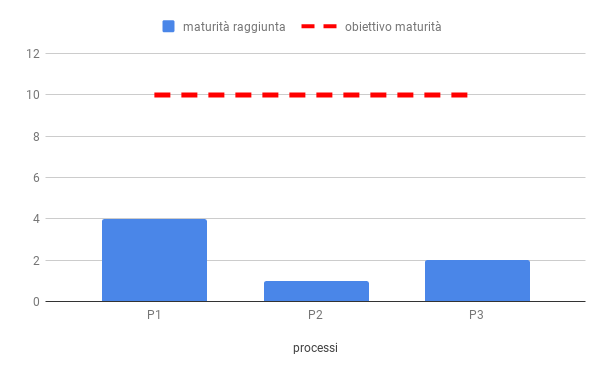
\includegraphics[scale=0.5]{MaturitaProcessi.png}
	\caption{Maturità macro-processi ISO 15504}
\end{figure}
\begin{itemize}
	\item \textbf{prc1:} processo gestito da automatismi, il gruppo sta imparando ad utilizzare quest'ultimi per rendere il lavoro più preciso e con meno possibilità di errore. Usando ad esempio toggle per il conteggio ore e integrazione slack con github tracciando le issue ha
	permesso di ottenere una migliore pianificazione;
	\item \textbf{proc2:} processo non ancora istanziato poichè non fa parte della revisione di requisit, abbiamo analizzato solo metriche in funzione degli obiettivi;
	\item \textbf{proc3:} processo non ancora istanziato, sarà comunque quasi completamente automatizzato
\end{itemize}
\clearpage
\subsubsection{Qualità di prodotto}
In questa fase ci si concentra principalmente sulla redazione dei documenti, pertanto le uniche metriche utilizzate sono quelle riguardanti i documenti.
Poichè, in particolari circostanze (non necessariamente rare), la valutazione automatica della leggibilità, se non tiene conto in alcun modo dei significati delle parole, può dare risultati inattendibili, per non dire fuorvianti si è scelto di non valutare i documenti tramite script che calcolano le metriche.
Nonostante cioò sono metriche puramente sintattiche, sono da considerare con la dovuta cautela \\
\href{https://docs.google.com/spreadsheets/d/1yMKJyV4I8FXQ7GUQOq8m1RdZeTYFTJ387ixzofNrfLI/edit?usp=sharing}{modifica grafici}\\
\href{https://www.webfx.com/tools/read-able/check.php?tab=Test+By+Url&uri=https%3A%2F%2Fwww.ispazio.net}{prova test leggibilità}
	 \\ \\
	Come si può notare dal trend dei grafici l'obiettivo è stato quasi sempre rispettato ottenendo dei documenti con una leggibilità media da istruzione superiore.
	\clearpage
\paragraph{Gunning Fog index}
\hspace{15cm}
\begin{figure}[h!]
	\centering
	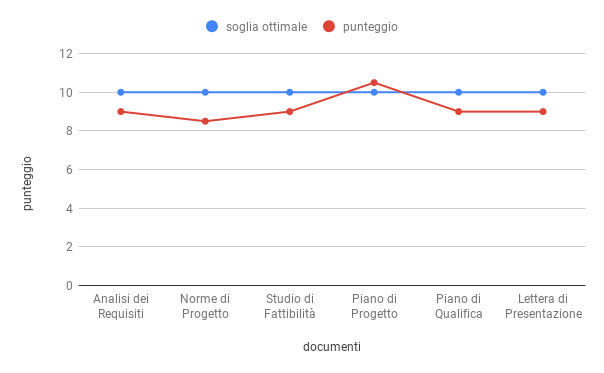
\includegraphics[scale=0.5]{GunningFogIndex.png}
	\caption{Gunning Fog index}

\end{figure}
%\clearpage
\paragraph{Simple Measure of Gobbledygook (SMOG)}
\hspace{15cm}
\begin{figure}[h!]
	\centering
	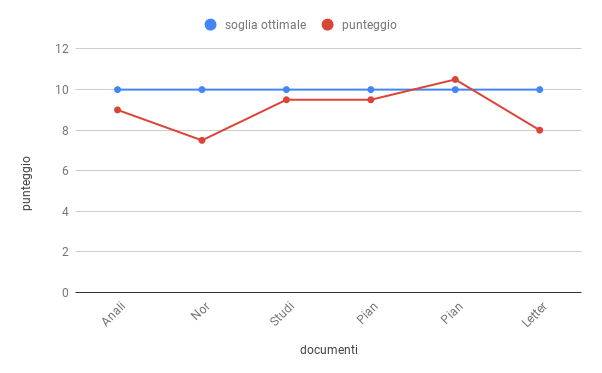
\includegraphics[scale=0.5]{Smog.png}
	\caption{SMOG}
\end{figure}
\clearpage
\paragraph{Gulpease Index}
\hspace{15cm}
\begin{figure}[h!]
	\centering
	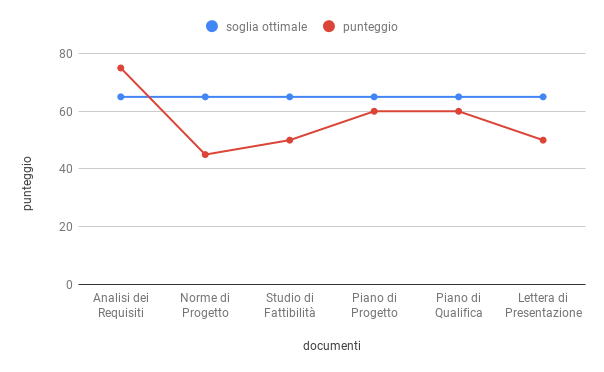
\includegraphics[scale=0.5]{GulpeaseIndex.png}
	\caption{Gulpease index}
\end{figure}

\paragraph{Errori sintattici}
\hspace{15cm}
 I verificatori hanno eliminato gli errori rimanenti presenti nei documenti, raggiungendo così il valore ottimale prefissato attraverso il software per il controllo ortografico presente in TexStudio. 
\subsubsection{Conclusioni}
Parlare se si è sforati nel budget (parlare quindi di metriche per il budget) e in quel caso perchè è successo.
\clearpage
\subsection{Revisione di Progettazione (RP)}
Questa sezione verrà riempita durante il periodo definito.
\subsection{Revisione di Qualifica(RQ)}
Questa sezione verrà riempita durante il periodo definito
\subsection{Revisione di Accettazione(RA)}
Questa sezione verrà riempita durante il periodo definito
\newpage
\end{document}
